
创建库的工作方式与创建可执行文件的方式类似,但因为库目标通常是由其他目标使用的,要么在同一个项目中,要么由其他项目使用。因为库通常有一个内部和公开可见的API,所以在向项目添加文件时必须考虑到这一点。

简单的库项目可以这样:

\begin{lstlisting}[style=styleCMake]
cmake_minimum_required(VERSION 3.21)

project(
	ch3.hello_lib
	VERSION 1.0
	DESCRIPTION
	"A simple C++ project to demonstrate creating executables
	and libraries in CMake"
	LANGUAGES CXX)
	
add_library(hello)

target_sources(
	hello
	PRIVATE src/hello.cpp src/internal.cpp)
	
target_compile_features(hello PUBLIC cxx_std_17)

target_include_directories(
	hello
	PRIVATE src/hello
	PUBLIC include)
\end{lstlisting}

同样,该文件以设置\texttt{cmake\_minimum\_required}和项目信息开始。

接下来,使用\texttt{add\_library}创建库的目标——本例中,库的类型没有确定。可以传递STATIC或SHARED来显式确定库的类型,这里可以省略设置该类型,我们允许库的使用者选择如何构建和链接。通常,静态库很容易处理。

若省略了库的类型,则BUILD\_SHARED\_LIBS将决定库是默认构建为动态库还是静态库。这个变量不应该在项目的CMake文件中设置,应该由构建者传递。

使用\texttt{target\_sources}为库添加源文件。第一个参数是目标名称,后面跟PRIVATE、PUBLIC或INTERFACE关键字分隔相应源文件。实践中,源文件使用PRIVATE添加,PRIVATE和PUBLIC关键字指定在何处使用源代码进行编译。PRIVATE指定的源文件将只在目标hello中使用。若使用PUBLIC,那么源文件也会将附加到hello和依赖hello的目标上,这通常不是我们想要的结果。INTERFACE关键字说明源文件不会添加到hello目标中,而是会添加到依赖到hello的目标上。通常,为目标指定为PRIVATE的内容都可以视为构建需求。最后,包含目录使用\texttt{target\_include\_directories}设置。该指令指定的文件夹内的所有文件都可以使用\#include <file.hpp>(带尖括号)来访问。

PRIVATE包含不会包含目标属性中的路径,也就是INTERFACE\_INCLUDE\_DIRECTORIES。当目标依赖于该库时,CMake将读取该属性以确定哪些包含目录可见。

由于标准库的C++代码使用了与现代版本C++绑定的特性,如C++11/14/17/20或C++23(即将发布),必须设置cxx\_std\_17属性。由于用于编译库本身并与需要其接口,因此将其设置为PUBLIC。只有在头文件包含需要特定标准的代码时,才需要将其设置为PUBLIC或INTERFACE。若只有内部代码依赖于某个标准,则首选将其设置为PRIVATE。通常,尽量将公共C++标准设置为最低的可用标准,也可以只启用现代C++标准的某些特性。

完整的可用编译特性列表可参阅\url{https://cmake.org/cmake/help/latest/prop_gbl/CMAKE\_CXX\_KNOWN\_FEATURES.html}。

\subsubsubsection{3.4.1\hspace{0.2cm}命名库}

当使用\texttt{add\_library(<name>)}创建库时,库名称在项目中必须全局唯一。默认情况下,库的实际文件名是根据平台上的约定构造的,例如lib<name>。在Linux上为<name>.lib,在Windows上为<名称>.dll。通过设置目标的OUTPUT\_NAME属性,可以更改文件的名称。可以在下面的例子中看到,输出文件的名称已经从ch3\_hello改为hello:

\begin{lstlisting}[style=styleCMake]
add_library(ch3_hello)

set_target_properties(
	ch3_hello
	PROPERTIES OUTPUT_NAME hello
)
\end{lstlisting}

避免使用lib前缀或后缀的库名称,因为CMake可能会在文件名后面或前面添加适当的字符串。当然,这取决于平台。

动态库的常用命名约定是在文件名中添加版本以指定构建版本和API版本,通过指定VERSION和SOVERSION属性,CMake将在构建和安装库时创建必要的文件名和符号链接:

\begin{lstlisting}[style=styleCMake]
set_target_properties(
	hello
	PROPERTIES VERSION ${PROJECT_VERSION} # Contains 1.2.3
	SOVERSION ${PROJECT_VERSION_MAJOR} # Contains only 1
)
\end{lstlisting}

Linux上,这个示例将会使libhello.so.1.0.0的文件名带有来自libhello的符号链接。所以,libhello.so.1指向实际的库文件。下面的截图展示了生成的文件和指向它的符号链接:

\begin{center}
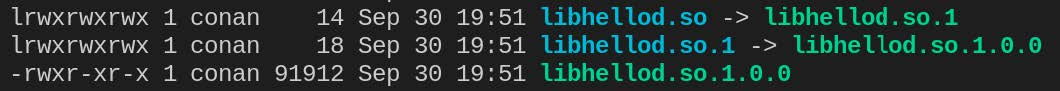
\includegraphics[width=1.\textwidth]{content/1/chapter3/images/1.jpg}\\
图3.1  使用SOVERSION属性构建库文件和生成的符号链接
\end{center}

项目中经常看到的另一种约定,是为各种构建配置的文件名添加不同的后缀。CMake通过设置CMAKE\_<CONFIG>\_POSTFIX全局变量或添加<CONFIG>\_POSTFIX属性来处理这个问题。若设置了此变量,后缀将自动添加到非可执行目标。与大多数全局变量一样,应该通过命令行传递给CMake,或者作为预置,而不是硬编码在CMakeLists.txt文件中。

调试库的后缀也可以显式地设置为单个目标,如下面的例子所示:

\begin{lstlisting}[style=styleCMake]
set_target_properties(
	hello
	PROPERTIES DEBUG_POSTFIX d)
\end{lstlisting}

这将使库文件和符号链接命名为libhellod。由于在CMake中链接库是针对目标而不是文件名进行的,因此会自动选择正确的文件名。然而,链接动态库时要注意的是符号可见性。

\subsubsubsection{3.4.2\hspace{0.2cm}动态库中的符号可见性}

要链接到动态库,链接器必须知道哪些符号可以从库外部使用。这些符号可以是类、函数、类型等,使它们可见的过程称为导出。

指定符号可见性时,编译器有不同的方式和默认行为,这使得以独立于平台的方式指定符号可见性有点麻烦。从默认的编译器可见性开始;gcc和clang假设所有的符号都是可见的,而Visual Studio编译器默认情况下会隐藏所有的符号,除非显式导出。设置CMAKE\_WINDOWS\_EXPORT\_ALL\_SYMBOLS,可以改变MSVC的默认行为,这是一种暴力的解决方法,只有当库的所有符号都应该导出时才能使用。

虽然将所有的符号设置为公共可见是确保链接容易的一种简单方法,但也有一些缺点:

\begin{itemize}
\item 
通过导出所有内容,就无法阻止依赖目标使用内部代码。

\item 
外部代码使用每个符号,链接器不能丢弃死代码,因此库体积往往会膨胀。若库中包含模板,则尤其如此,因为模板往往会大幅增加符号的数量。

\item 
由于导出了每个符号,关于哪些应该隐藏或内部符号的唯一线索必须来自文档。

\item 
暴露库的内部符号会暴露本应隐藏的东西。

\begin{tcolorbox}[colback=blue!5!white,colframe=blue!75!black,title=所有符号可见]
将动态库中的所有符号设置为可见时要小心,特别是在关心安全问题或二进制文件的大小很重要时。
\end{tcolorbox}
\end{itemize}

\hspace*{\fill} \\ %插入空行
\noindent
\textbf{更改默认可见性}

要更改符号的默认可见性,请将\texttt{<LANG>\_VISIBILITY\_PRESET}属性设置为\texttt{HIDDEN}。此属性可以全局设置,也可以针对单个库目标设置。\texttt{<LANG>}会替换为编写库的语言,例如:CXX替换为C++, C替换为C。若所有要导出的符号都是隐藏符号,必须在代码中特别标记。最常见的方法是指定一个预处理器定义来确定一个符号是否可见:

\begin{lstlisting}[style=styleCXX]
class HELLO_EXPORT Hello {
	…
};
\end{lstlisting}

HELLO\_EXPORT将包含这样的信息:当编译库时,该符号是否导出,或者当对库进行链接时,它是否应该导入。GCC和Clang使用\_\_attribute\_\_(…)关键字来确定此行为,而在Windows上使用\_declspec(…)。编写以跨平台方式处理此问题的头文件并不是一项轻松的任务,特别是若还要考虑库可能构建为静态库和对象库。幸运的是,CMake提供了\texttt{generate\_export\_header}宏,由\texttt{GenerateExportHeader}模块导入。

下面的例子中,hello库的符号默认设置为隐藏。然后,通过使用\texttt{generate\_export\_header}宏再次单独启用。另外,本例将VISIBILITY\_INLINES\_HIDDEN属性设置为TRUE,通过隐藏内联类成员函数进一步减少导出的符号表。并不严格要求设置内联的可见性,但通常在设置了默认可见性后才会这样做:

\begin{lstlisting}[style=styleCMake]
add_library(hello SHARED)
set_property(TARGET hello PROPERTY CXX_VISIBILITY_PRESET "hidden")
set_property(TARGET hello PROPERTY VISIBILITY_INLINES_HIDDEN TRUE)
include(GenerateExportHeader)
generate_export_header(hello EXPORT_FILE_NAME export/hello/	export_hello.hpp)

target_include_directories(hello PUBLIC "${CMAKE_CURRENT_BINARY_DIR}/export")
\end{lstlisting}

\texttt{generate\_export\_header}的调用在CMAKE\_CURRENT\_BINARY\_DIR/export/hell目录中创建了一个名为export\_hello.hpp的文件,该文件可以包含在库的文件中。将这些生成的文件放在构建目录的子文件夹中是一个好做法,这样只将目录的一部分添加到包含路径中。生成文件的include结构应该与库的其他部分的include结构匹配。在这个例子中,通过\#include <hello a\_public\_header.h>来包含所有公共头文件,那么导出头文件也应该放在名为hello的文件夹中。生成的文件也必须添加到安装说明中。此外,要创建导出文件,必须将用于导出符号的必要编译器标志设置为目标。

因为生成的头文件必须包含在声明要导出的类、函数和类型的文件中,所以CMAKE\_CURRENT\_BINARY\_DIR/export/添加到\texttt{target\_include\_directories}中。注意,必须是PUBLIC,这样依赖库才可以找到该文件。

关于\texttt{generate\_export\_header}宏还有很多选项,但本节中看到的内容涵盖了大多数用例。关于设置符号可见性的其他信息,可以查阅官方CMake文档\url{https://cmake.org/cmake/help/latest/module/GenerateExportHeader.html}。

\subsubsubsection{3.4.3\hspace{0.2cm}接口或纯头文件库}

纯头文件的库有点特殊,因为不需要编译;相反,可以导出它们的头文件,以便直接包含在其他库中。大多数情况下,头文件库的工作方式与普通库类似,但是头文件使用INTERFACE,而非PUBLIC。

由于仅包含头文件的库不需要编译,因此不会向目标添加源文件。下面的代码创建了一个小的纯头文件库:

\begin{lstlisting}[style=styleCMake]
project(
	ch3_hello_header_only
	VERSION 1.0
	DESCRIPTION "Chapter 3 header-only example"
	LANGUAGES CXX)

add_library(hello_header_only INTERFACE)
target_include_directories(hello_header_only INTERFACE include/)
target_compile_features(hello_header_only INTERFACE cxx_std_17)
\end{lstlisting}

CMake 3.19版本之前,INTERFACE库不能使用\texttt{target\_sources}。现在,纯头文件库可以不列出源文件。

\hspace*{\fill} \\ %插入空行
\noindent
\textbf{对象库——仅供内部使用}

有时,可能想要分离代码,以便部分代码可以重用,而不需要创建完整的库。当想在可执行测试和单元测试中使用某些代码时,通常的做法是不需要重新编译所有代码两次。为此,CMake提供了对象库,其中的源代码是编译的,但不进行归档或链接。通过\texttt{add\_library(MyLibrary object)}创建对象库。

自CMake 3.12起,这些对象可以像普通库一样使用,只需将它们添加到\texttt{target\_link\_libraries}函数中。3.12版本之前,对象库需要添加生成器表达式,也就是\$<TARGET\_OBJECTS:MyLibrary>。这将在生成构建系统期间扩展为一个对象列表。这种方式现在还可以用,但不推荐这样做,因为这很快就变得不可维护,特别是在一个项目中有多个对象库的情况下。

\begin{tcolorbox}[colback=blue!5!white,colframe=blue!75!black,title=何时使用对象库]
对象库可以在不公开模块的情况下加快代码的构建和模块化。
\end{tcolorbox}

使用对象库,可以覆盖所有不同类型的库。编写和维护库本身很有趣,但除非将其集成到更大的项目中,否则它们什么也做不了。那么,让我们看看如何在可执行文件中,使用目前定义的库。








